% Hypothetical fixed reward pool V_{\mathrm{pool}}, honest work U_{\mathrm{honest}} > 0, no prior attacker work.
% r_self = u_self / U_honest; a = full self-purchase cost per work * U_honest / V_pool.
% Normalized incremental payoff is r_self/(1+r_self) - a*r_self.
% PGFPlots' internal variable x represents r_self. No token-price forecast.
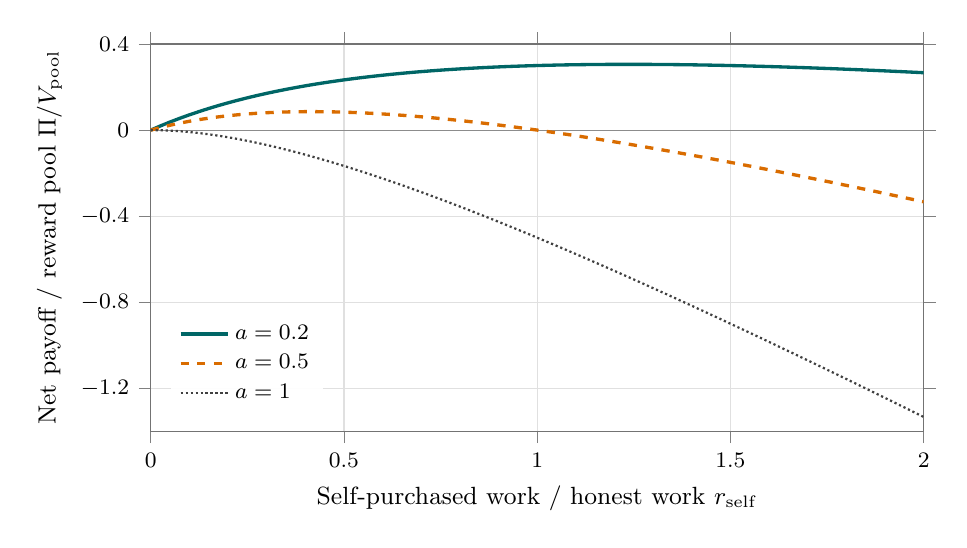
\begin{tikzpicture}
\begin{axis}[
  width=.94\linewidth, height=6.5cm,
  xmin=0, xmax=2, ymin=-1.4, ymax=.4,
  xlabel={Self-purchased work / honest work \(r_{\mathrm{self}}\)},
  ylabel={Net payoff / reward pool \(\Pi/V_{\mathrm{pool}}\)},
  xtick={0,.5,1,1.5,2},
  ytick={-1.2,-.8,-.4,0,.4},
  grid=major, grid style={black!12},
  tick align=outside, axis line style={black!55},
  font=\small, tick label style={font=\footnotesize},
  label style={font=\small},
  legend style={at={(.025,.045)}, anchor=south west, draw=none,
    fill=white, fill opacity=.95, text opacity=1, font=\footnotesize,
    cells={anchor=west}},
  clip=true,
]
\addplot[black!45, thin, forget plot] coordinates {(0,0) (2,0)};
\addplot[teal!80!black, very thick, domain=0:2, samples=81] {x/(1+x)-.2*x};
\addlegendentry{\(a=0.2\)}
\addplot[orange!85!black, very thick, dashed, domain=0:2, samples=81] {x/(1+x)-.5*x};
\addlegendentry{\(a=0.5\)}
\addplot[black!75, thick, densely dotted, domain=0:2, samples=81] {x/(1+x)-x};
\addlegendentry{\(a=1\)}
\end{axis}
\end{tikzpicture}
